\documentclass[11pt]{article}
\usepackage{fontspec}
\setmainfont{Arial}
\setsansfont{Arial}
\setmonofont{DejaVu Sans Mono}[Scale=MatchLowercase]
\usepackage[margin=1in]{geometry}
\usepackage{amsmath,amssymb}
\usepackage{graphicx}
\usepackage{booktabs}
\usepackage{array}
\usepackage{multirow}
\usepackage{siunitx}
\usepackage{caption}
\usepackage{subcaption}
\usepackage{placeins}
\usepackage{tikz}
\usetikzlibrary{arrows.meta,positioning,calc,fit,decorations.pathreplacing}
\usepackage[numbers,round]{natbib}
\usepackage[svgnames]{xcolor}
\usepackage{authblk}
\usepackage{microtype}
\usepackage{xurl}
\usepackage[hidelinks]{hyperref}

\captionsetup{font=small,labelfont=bf}
\setlength{\parskip}{0.3em plus 0.1em minus 0.05em}
\setlength{\parindent}{0pt}
\setlength{\emergencystretch}{1em}
\setlength{\textfloatsep}{10pt plus 3pt minus 3pt}
\setlength{\floatsep}{9pt plus 2pt minus 2pt}
\setlength{\intextsep}{9pt plus 2pt minus 2pt}
\renewcommand{\topfraction}{0.9}
\renewcommand{\bottomfraction}{0.85}
\renewcommand{\textfraction}{0.08}
\renewcommand{\floatpagefraction}{0.72}
\setcounter{topnumber}{3}
\setcounter{bottomnumber}{2}
\setcounter{totalnumber}{4}
\makeatletter
\setlength{\@fptop}{0pt}
\setlength{\@fpsep}{10pt plus 2pt}
\setlength{\@fpbot}{0pt plus 1fil}
\makeatother
\raggedbottom

\newcommand{\panfig}[1]{\resizebox{\textwidth}{!}{\input{#1}}}
\newcommand{\panhalffig}[1]{\resizebox{0.98\linewidth}{!}{\input{#1}}}

\graphicspath{{journal-figures/}{standalone-assets/}{tikz/}{./}}
\newcommand{\figpanel}[2]{Figure~\hyperref[#1]{\ref*{#1}#2}}
\newcommand{\InventoryFiles}{1587}
\newcommand{\LatentFiles}{1585}
\newcommand{\UniqueScores}{1236}
\newcommand{\NativeFiles}{910}
\newcommand{\NonNativeFiles}{675}
\newcommand{\ValidNativeFiles}{855}
\newcommand{\GuardedNativeFiles}{55}
\newcommand{\NullEligible}{60}
\newcommand{\NullCoherence}{59}
\newcommand{\NullJoint}{57}
\newcommand{\MaxExactDelta}{0.066412}

\hypersetup{pdftitle={Reference-anchored diagnostics of single-cell geometry and native allocation coherence},pdfauthor={Zeyu Fu}}
\title{Reference-anchored diagnostics of single-cell geometry and native allocation coherence}
\author[1]{Zeyu Fu*}
\affil[1]{\hspace{0.2em}State Key Laboratory of Trauma and Chemical Poisoning, Institute of Combined Injury,
Chongqing Engineering Research Center for Nanomedicine, College of Preventive Medicine,
Army Medical University, Chongqing, China\\\texttt{fuzeyu09@gmail.com}}
\date{}
\begin{document}\maketitle
\section*{Supplementary Information}
\renewcommand{\thefigure}{S\arabic{figure}}\renewcommand{\thetable}{S\arabic{table}}
\begin{figure}[!b]
\centering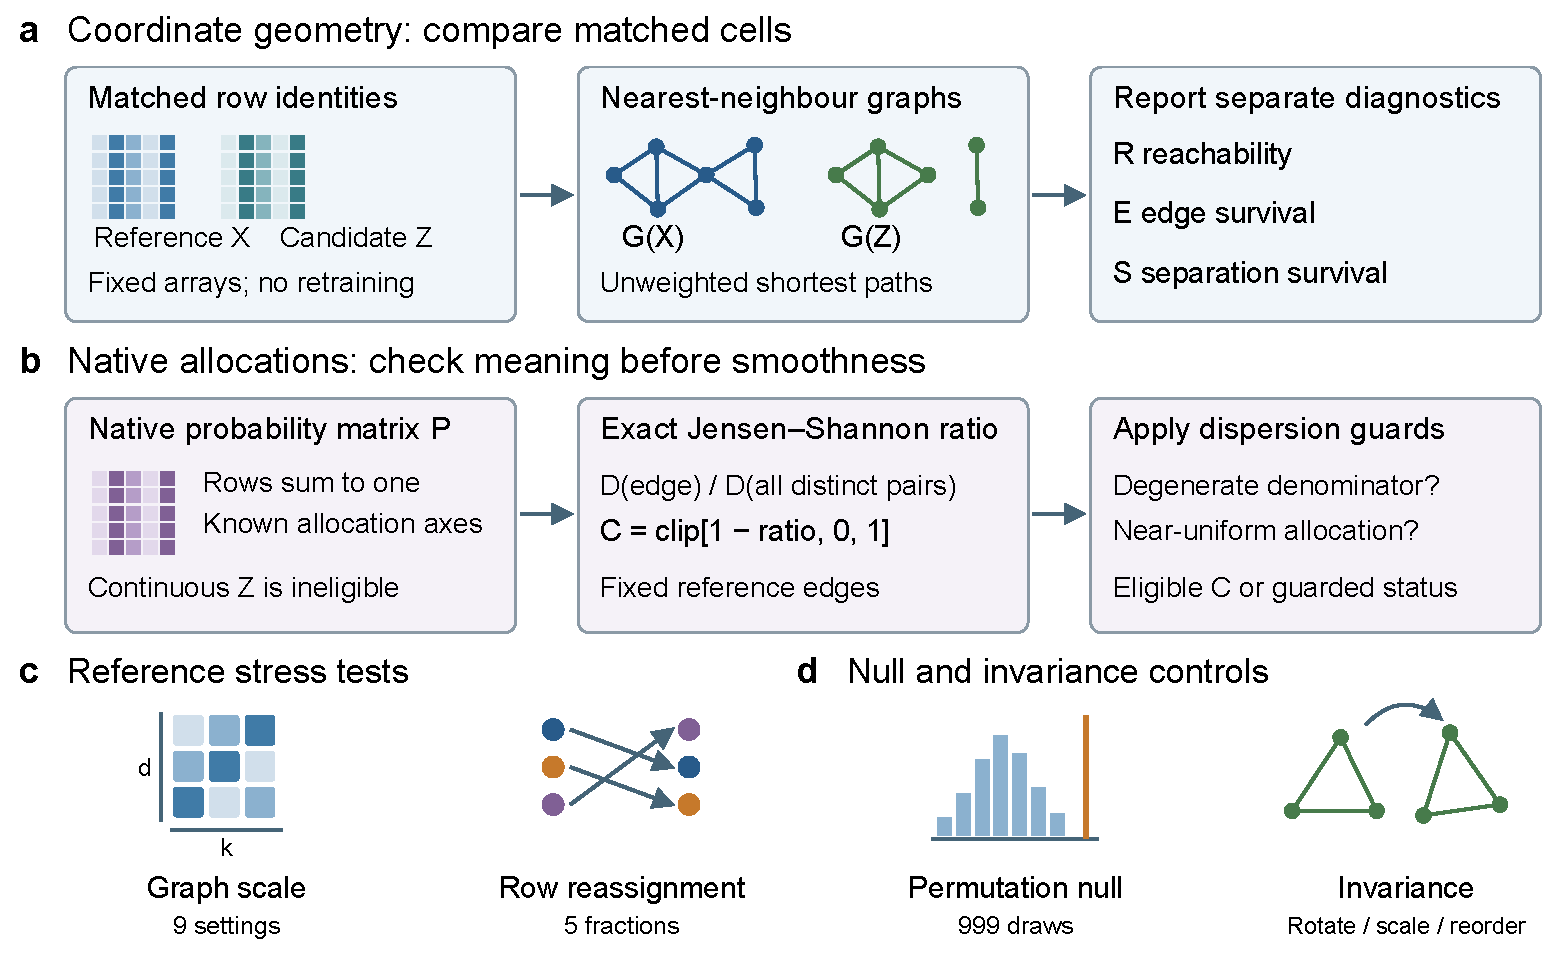
\includegraphics[width=\linewidth]{journal-figures/architecture.pdf}
\caption{Measurement modules and fixed-object probes. a, matched reference and candidate rows generate separate undirected nearest-neighbour graphs; shortest paths supply reachability $R$, edge survival $E$ and separation $S$. b, a model-declared native probability matrix supplies Jensen--Shannon divergences on reference edges and over all distinct pairs; denominator and dispersion guards determine whether coherence is quotable. Continuous coordinates stop before this pathway. c, reference stress tests cross neighbour counts $k=5,15,30$ with PC counts $d=10,25,50$ and vary selected-row fractions over 0, 10, 25, 50 and 100\%. d, controls include the 999-draw permutation comparison and rotation, rescaling and joint reordering. Grid tiles, reassignment arrows, histogram bars and graph nodes are illustrative, not additional measurements, data distributions or inferred biological modules.}
\label{fig:workflow}
\end{figure}

\begin{table}[!ht]
\centering\small
\caption{Seed-42 calibration, with matched noise and $k=15$. Shatter uses amplitude 2.5; collapse retains zero fork coordinate. Values come directly from the named implementation. The official trajectory row must not be identified with the local surrogate.}
\label{tab:calibration}
\begin{tabular}{lrrrr}
\toprule
Metric & Faithful & Shatter & Collapse & Permuted \\
\midrule
Trustworthiness & 0.9974 & 0.9970 & 0.7997 & 0.5084 \\
LCMC (zadu) & 0.7718 & 0.7685 & 0.4924 & 0.0011 \\
Local root-geodesic surrogate & 0.9997 & 0.9983 & 0.9994 & 0.4850 \\
scIB graph connectivity & 1.0000 & 1.0000 & 0.9200 & 0.4378 \\
scIB trajectory conservation & 0.9943 & 0.0960 & 0.5272 & 0.5114 \\
RAAG reachability & 1.0000 & 0.3318 & 1.0000 & 1.0000 \\
RAAG edge survival & 0.9214 & 0.9065 & 0.7456 & 0.1465 \\
RAAG separation & 1.0000 & 1.0000 & 0.6952 & 0.5357 \\
\bottomrule
\end{tabular}

\end{table}

\begin{figure}[!ht]
\centering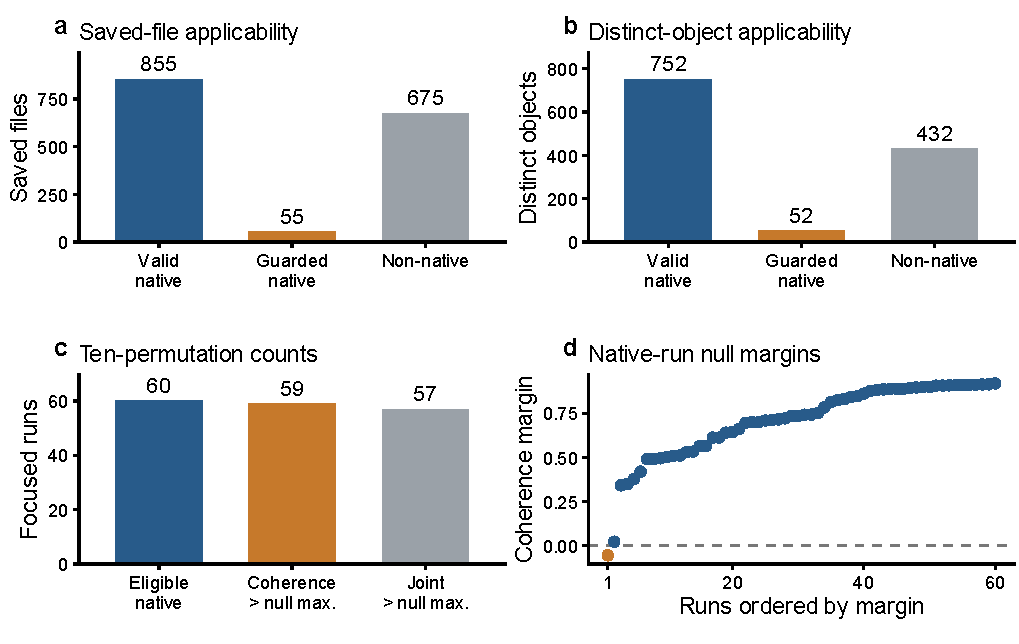
\includegraphics[width=\linewidth,height=0.64\textheight,keepaspectratio]{journal-figures/inventory_null_comparison.pdf}
\caption{Applicability, computational identity and descriptive permutation comparisons. a, all \LatentFiles{} saved latent files, including aliases: valid native, guarded native and non-native continuous outputs. b, the corresponding \UniqueScores{} distinct computational objects after deduplication; the same categories retain 752, 52 and 432 objects. c, the separate 144-run focused manifest: 60 eligible native runs, 59 whose coherence exceeds all ten row permutations, and 57 exceeding their maxima jointly for edge survival, separation and coherence. Bar positions and annotations give counts; denominators differ between panels. d, all 60 native-run margins, observed coherence minus the maximum of that run's ten permuted coherence values, ordered from lowest to highest. The dashed line is zero margin; the nonpositive comparison is orange and positive margins blue. Each point is a computational run, not a biological replicate. Positive margins do not establish 5\% Monte Carlo significance: the smallest corrected permutation probability with ten draws is $1/11$. Repeated files, seeds and checkpoints do not add independent biological units.}
\label{fig:coverage}
\end{figure}

\begin{figure}[!b]
\centering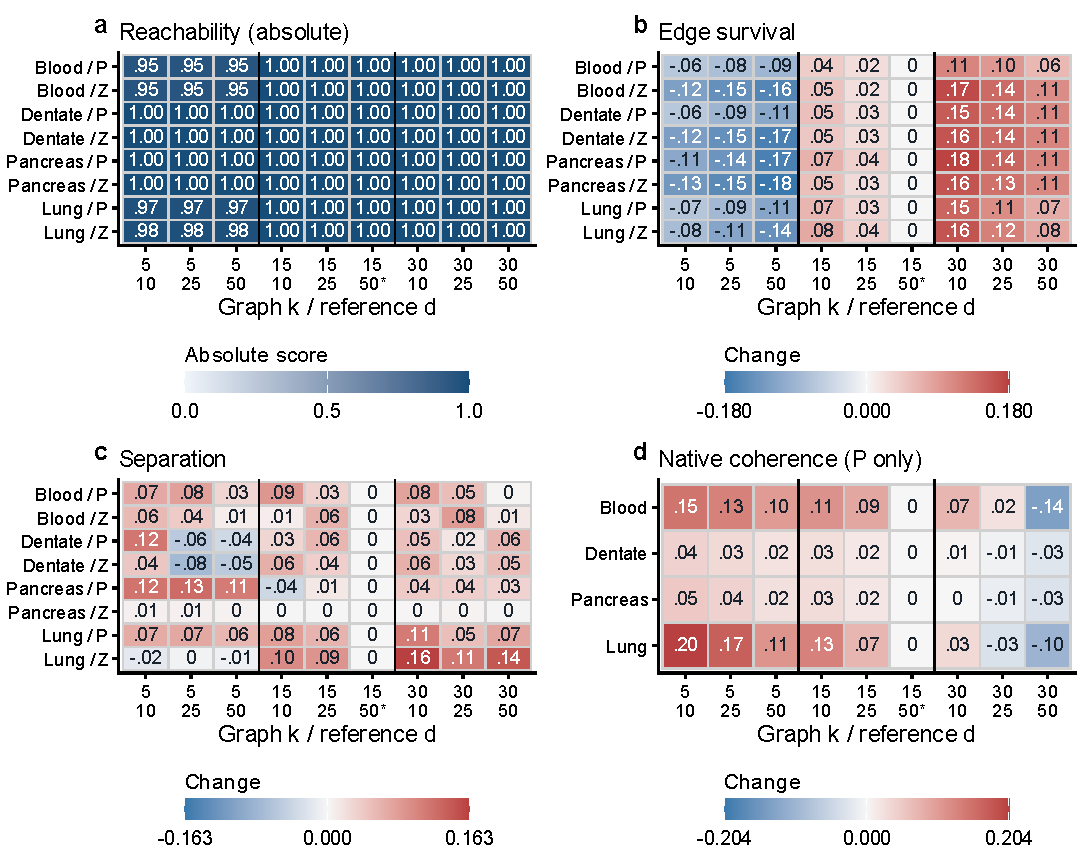
\includegraphics[width=\linewidth,height=0.64\textheight,keepaspectratio]{journal-figures/scale_reference_sensitivity.pdf}
\caption{Sensitivity to graph scale and reference dimension for fixed candidate arrays. a, absolute reference-connected-pair reachability on a zero-to-one scale; 1.00 means that every pair connected in the reference remains connected in the candidate, not that row correspondence or local geometry is preserved. Values near one therefore expose saturation of this connectivity diagnostic. b, edge-survival change. c, separation change. d, native-coherence change, restricted to native probability inputs. Each tile averages three stored seeds. Panels b--d subtract the same objects' $k=15,d=50$ baseline and retain separate symmetric colour scales; zero is no change, including the baseline by construction. Annotations are rounded to two decimals, and changes below 0.005 in magnitude display as zero; colour retains the full value. Two-line columns give neighbour count $k$ above reference PC count $d$, vertical rules separate $k$ groups, and the asterisk marks baseline. Rows identify blood, dentate, pancreas and lung; P denotes native probabilities and Z continuous coordinates in a--c. Continuous rows are omitted only from d because native coherence is undefined for them. The 10- and 25-PC references truncate the stored 50-PC reference without refitting. Colours cannot be compared quantitatively across panels, and signs do not select preferred settings. Repeated settings and stored seeds are not biological replication units.}
\label{fig:scale}
\end{figure}

\begin{figure}[!b]
\centering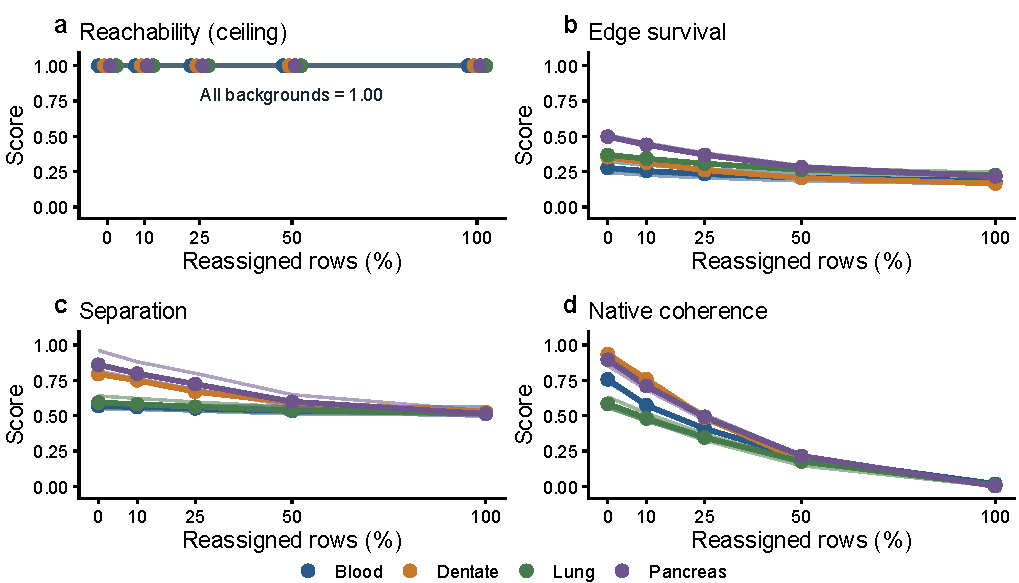
\includegraphics[width=\linewidth,height=0.64\textheight,keepaspectratio]{journal-figures/row_correspondence_sensitivity.pdf}
\caption{Sensitivity to disrupted cell correspondence at $k=15$ and 50 reference PCs. a, reachability; the single grey line is intentional because every background and every reassignment fraction has an exact score of 1.00, while small coloured horizontal offsets separate the coincident background markers for visibility. b, edge survival. c, separation. d, native allocation coherence. The single colour key below the panels identifies the four backgrounds throughout the figure. Thick curves and points average three stored model seeds and three corruption seeds within each background; faint curves retain individual model seeds after averaging their three corruption seeds. The horizontal axis gives the selected row fraction at the five tested levels, 0, 10, 25, 50, and 100\%, rounded down to an integer cell count. Selected allocation rows are reassigned in one cycle, preserving their marginal distribution; each changes identity when at least two rows are selected. Repeated zero-fraction controls add no independent observations. Lines connect the tested fractions without fitting a response model. No error bars or population-level inference are implied, and the retained model-seed curves need not decline monotonically.}
\label{fig:correspondence}
\end{figure}

\begin{table}[!t]
\centering\small
\caption{Edge survival against tissue position. Values are rounded to three decimals. The permutation reorders PCA rows. Each row is one section.}
\label{tab:spatial}
\begin{tabular}{lrrrrr}
\toprule
Object & PCA & scVI & UMAP & Random & Permuted \\
\midrule
Olfactory bulb (262) & 0.514 & 0.517 & 0.315 & 0.504 & 0.453 \\
PFC 151673 (3{,}639) & 0.460 & 0.424 & 0.208 & 0.319 & 0.337 \\
Liver metastasis (1{,}184) & 0.579 & 0.625 & 0.416 & 0.433 & 0.306 \\
PFC 151507 (4{,}226) & 0.437 & 0.389 & 0.165 & 0.301 & 0.362 \\
Lymph node (4{,}035) & 0.435 & 0.415 & 0.200 & 0.309 & 0.296 \\
Breast cancer (3{,}798) & 0.501 & 0.532 & 0.269 & 0.334 & 0.270 \\
Ovarian cancer (3{,}493) & 0.441 & 0.428 & 0.186 & 0.319 & 0.316 \\
\bottomrule
\end{tabular}

\end{table}

\begin{figure}[!p]
\centering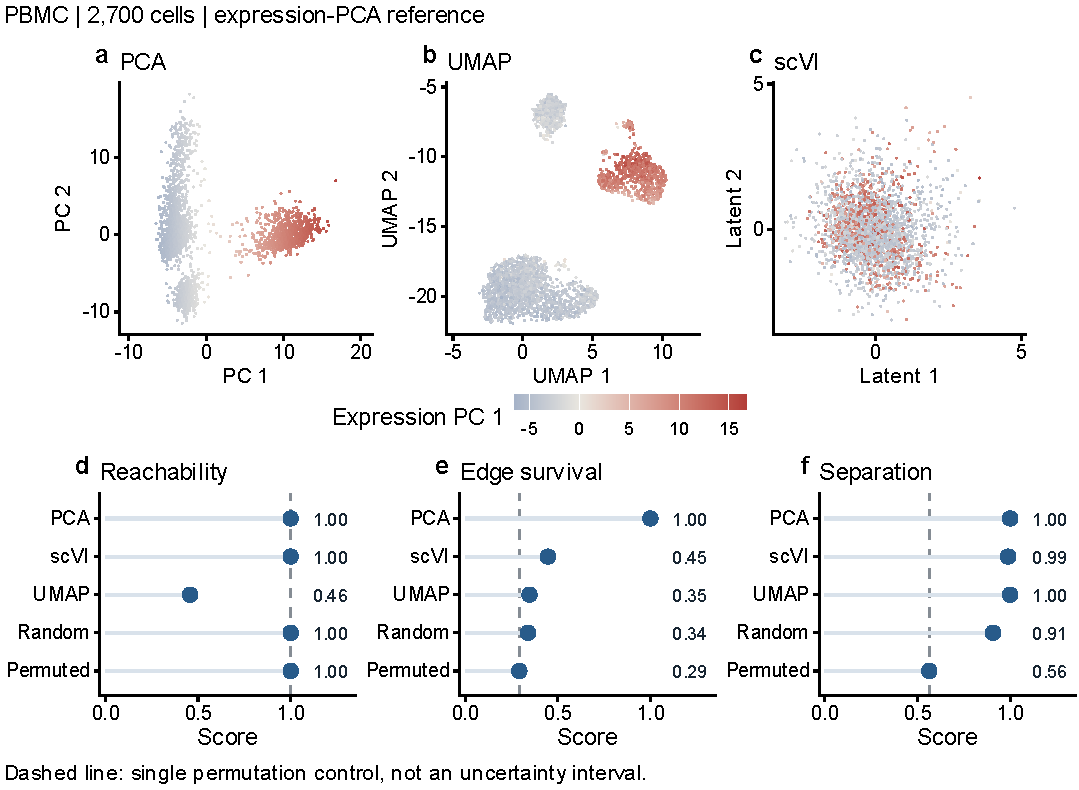
\includegraphics[width=\linewidth,height=0.65\textheight,keepaspectratio]{journal-figures/object_pbmc.pdf}
\caption{PBMC coordinate views and complementary preservation scores for one 2,700-cell object without tissue positions. a, the first two expression PCs. b, UMAP. c, the first two scVI latent dimensions. Coordinate views use equal aspect, separate limits, and a shared expression-PC-1 colour scale. d, separately saved reachability against the 50-PC expression reference. e, edge survival. f, separation. All five evaluated candidates are retained, including random projection and one PCA-row permutation. Points and two-decimal annotations report fixed-object scores; a reachability value of 1.00 is the connected-pair ceiling and does not certify row correspondence. Dashed lines mark the metric-specific permutation value, not a significance threshold. PCA is an identity control for this reference, rather than an independently successful method. The displayed scVI coordinates come from a visualization refit and are not the scored array. No native-allocation claim, uncertainty interval, lineage inference, or donor-level replication is implied.}
\label{fig:pbmc}
\end{figure}

\begin{table}[!ht]
\centering\small
\caption{Edge survival against the expression PCA. The PCA column is 1 by construction. PBMC has no tissue coordinate. Values are rounded to three decimals.}
\label{tab:expression}
\begin{tabular}{lrrrrr}
\toprule
Object & PCA & scVI & UMAP & Random & Permuted \\
\midrule
Olfactory bulb (262) & 1.000 & 0.643 & 0.642 & 0.541 & 0.453 \\
PFC 151673 (3{,}639) & 1.000 & 0.421 & 0.265 & 0.327 & 0.336 \\
Liver metastasis (1{,}184) & 1.000 & 0.567 & 0.606 & 0.451 & 0.305 \\
PFC 151507 (4{,}226) & 1.000 & 0.382 & 0.218 & 0.311 & 0.361 \\
Lymph node (4{,}035) & 1.000 & 0.516 & 0.377 & 0.319 & 0.296 \\
Breast cancer (3{,}798) & 1.000 & 0.569 & 0.465 & 0.343 & 0.269 \\
Ovarian cancer (3{,}493) & 1.000 & 0.495 & 0.343 & 0.327 & 0.314 \\
PBMC (2{,}700) & 1.000 & 0.447 & 0.347 & 0.339 & 0.292 \\
\bottomrule
\end{tabular}

\end{table}

\section*{Supplementary Note: Extended discussion}

The experiments support a conditional interpretation of geometric fidelity, and they show that the condition has to include the chance level of each score. Matching the starting noise removed an apparent local-score improvement under arm separation, and direct execution of the official trajectory API gave a strong shatter response that the local root-distance surrogate did not reproduce; those corrections address experimental confounding and implementation misidentification. Two further corrections change what the diagnostics can claim. With a connected reference, reachability does not use the reference at all: it is the fraction of candidate pairs in the same candidate component, which detects gaps wider than the neighbour radius but ignores merging and is matched or exceeded in sensitivity by distance-rank and global-structure scores. And raw edge survival compares candidates on different chance scales, because hop distances depend on the density and dimension of each candidate graph.

The second correction reverses several comparisons. Scored against its own permutation, UMAP retained tissue neighbourhoods above chance in edge survival on every section, and scVI matched or exceeded PCA on all seven fixed arrays, whereas raw edge survival placed PCA higher on four of the seven. Most of the change of edge survival with neighbour count was the rising chance floor; what remained was still material and should be reported with the chosen setting. Corrected tissue-reference edge survival was stable across refits (standard deviation at most 0.0066) and associated with candidate-neighbour purity of externally annotated cortical layers; corrected separation was not similarly stable. This is descriptive evidence on the same tissue objects, not independent biological validation: each section contributes twelve nonpermuted arrays, several of them seeds of the same method, and only two sections are available. A tie-aware rank statistic such as far-versus-edge AUROC avoids the candidate-median threshold's inflated chance level, but still needs a complementary fragmentation check.

The same reasoning applies to allocation coherence. Native allocations exceeded random smooth and raw mixture baselines everywhere, but a mixture fitted to the reference and tempered to the same sharpness came close and exceeded them in lung. Coherence is a Geary-type smoothness ratio on the reference graph, so a high value is expected of any allocation that varies smoothly with expression; the informative quantity is its margin over a baseline of matched sharpness.

Exact coherence improves one narrower aspect of reproducibility. Its denominator is a property of all distinct allocation pairs and therefore does not depend on which row positions happened to enter a random sample. For the stored tie-free objects, joint-reordering controls differ by at most floating-point accumulation, and rotation with uniform rescaling preserves geometry scores. The exact-tie probe exposes a concrete exception: arbitrary neighbour membership and positional self-removal break the expected graph invariance under coordinate collapse. The identity-explicit rescoring agrees with all 444 archived batteries, but it does so on tie-free objects where its tie rule is never used, so it does not test that rule on tied data. This numerical agreement therefore cannot be extended to arbitrary tie-breaking rules or representations. An exact ratio can still describe a scientifically uninformative object. The independently checked tail fixture shows that coherence can remain high while absolute allocation variation becomes extremely small yet remains above the numerical guard. A concentrated, almost constant allocation need not trigger the near-uniform guard. Native semantics, denominator eligibility and perplexity are therefore necessary reporting checks, not sufficient evidence of biological usefulness. Absolute divergence and total variation should accompany the relative score; a practically useful contrast requires an external target rather than another numerical threshold chosen from these fixtures.

The stored-data census illustrates the importance of that eligibility denominator. Continuous coordinates, native allocations, guarded allocations, duplicate files, and repeated checkpoints all occur in the available collection. Counting them together would change the population being described and could create artificial precision. Our focused permutation comparison accordingly reports the eligible native population, while the full inventory retains every alias for provenance. Ten permutations yield a minimum possible Monte Carlo probability of one eleventh when the observed arrangement is included~\cite{phipson2010permutation}; an above-maximum count is therefore a descriptive comparison. Neither a large file count nor repeated optimizer seeds creates additional biological replication.

Several design choices remain limitations of this measurement study. The archived calibration used identical reference and faithful noise draws; the graded calibration decoupled them and added three topologies without changing the conclusions, but all fixtures remain planar and noiseless in expression. The low official trajectory value of the identity control reflects the stability of diffusion pseudotime on a nearly noise-free planar graph rather than root selection, and exact distance ties in the tissue reference changed none of the reported orderings. The reference was always the 15-neighbour union graph of tissue positions or expression components; other reference graphs, such as distance-threshold graphs, were not tested. The fixed real-data subset covers four backgrounds and three stored seeds per representation type, selected by configuration rather than outcome. Those objects are not a representative sample of all embedding algorithms, biological tissues, or training budgets. Their expression references preserve the historical transductive preprocessing and PCA fitting procedure. Consequently, the observed sensitivity cannot be interpreted as a test of generalization to cells excluded from every preprocessing step. The diversity extension uses seven tissue sections and one blood matrix, with PCA, scVI, UMAP, a random projection, and one row permutation. Edge survival still depends on which reference is declared. It does not turn these objects into a donor-level sample.

The practical implication is to make evaluation records more explicit. A reusable result should retain matched row identities, the reference construction, graph settings, the semantic type of the candidate, implementation versions, and unavailable or guarded outputs. The separate diagnostics then permit a reader to distinguish a loss of connectedness from local distortion, altered separation, or reduced allocation variation. Preserving those distinctions is also useful when a metric behaves unexpectedly: the investigator can revisit the responsible object or intervention instead of treating a composite score as a complete verdict. The accompanying source package includes the selected arrays and executable sensitivity analyses so that these relationships can be examined directly.

Biological validity needs an external target of its own. Count simulators such as Splatter~\cite{zappia2017splatter} and dynamic simulators such as dyngen~\cite{cannoodt2021dyngen} would extend the planar fixtures to realistic expression with known topology, and clonal lineage measurements~\cite{weinreb2020lineage} could test whether a corrected geometric score predicts observed fate. The present results establish three practical requirements for any such test: report each score against its candidate-specific null, evaluate it alongside established comparators under the same interventions, and compare allocation scores with a baseline of matched smoothness.


\FloatBarrier
\bibliographystyle{unsrtnat}
\bibliography{references}
\end{document}